\documentclass[11pt]{article}

\usepackage[margin=1in]{geometry}
\usepackage[T1]{fontenc}
\usepackage{lmodern}
\usepackage{microtype}
\usepackage{amsmath,amssymb,amsthm,mathtools}
\usepackage{mathrsfs}
\usepackage[dvipsnames]{xcolor}
\usepackage[most]{tcolorbox}
\usepackage{tikz}
\usetikzlibrary{decorations.markings}
\usepackage{enumitem}
\usepackage{tocloft}
\usepackage[hidelinks]{hyperref}

\definecolor{courseblue}{HTML}{1F4E79}
\definecolor{lightblue}{HTML}{EAF2F8}
\definecolor{lightgreen}{HTML}{EAF7EA}
\definecolor{lightpink}{HTML}{FCE8EF}
\definecolor{lightyellow}{HTML}{FFF8D6}
\definecolor{warningyellow}{HTML}{D6A000}
\definecolor{exercisebg}{HTML}{FDEAEA}
\definecolor{exerciseframe}{HTML}{B54040}
\definecolor{examplebg}{HTML}{F4FAFE}
\definecolor{exampleframe}{HTML}{85C1E9}
\definecolor{darkgray}{HTML}{333333}
\definecolor{lightorange}{HTML}{FDEBD8}
\definecolor{orangeframe}{HTML}{E08A3C}

\setlength{\parindent}{0pt}
\setlength{\parskip}{0.65em}
\setlist[itemize]{topsep=0.25em,itemsep=0.15em}
\renewcommand{\cftsecleader}{\cftdotfill{\cftdotsep}}
\renewcommand{\cftsubsecleader}{\cftdotfill{\cftdotsep}}

\theoremstyle{plain}
\newtheorem{theorem}{Theorem}[section]
\newtheorem{proposition}[theorem]{Proposition}
\newtheorem{lemma}[theorem]{Lemma}
\newtheorem{corollary}[theorem]{Corollary}
\theoremstyle{definition}
\newtheorem{definition}[theorem]{Definition}
\newtheorem{example}[theorem]{Example}
\newtheorem{exercise}[theorem]{Exercise}
\theoremstyle{remark}
\newtheorem*{remark}{Remark}
\newtheorem*{fact}{Fact}
\newtheorem*{warning}{Warning}

\tcolorboxenvironment{definition}{
  enhanced,
  unbreakable,
  colback=lightgreen,
  colframe=ForestGreen,
  boxrule=0.7pt,
  arc=2pt,
  left=6pt,
  right=6pt,
  top=5pt,
  bottom=5pt
}

\tcolorboxenvironment{warning}{
  enhanced,
  colback=lightyellow,
  colframe=warningyellow,
  boxrule=0.7pt,
  arc=2pt,
  left=6pt,
  right=6pt,
  top=5pt,
  bottom=5pt
}

\tcolorboxenvironment{exercise}{
  enhanced,
  colback=exercisebg,
  colframe=exerciseframe,
  boxrule=1pt,
  arc=2pt,
  left=6pt,
  right=6pt,
  top=5pt,
  bottom=5pt
}

\tcolorboxenvironment{example}{
  enhanced,
  colback=examplebg,
  colframe=exampleframe,
  boxrule=0.7pt,
  arc=2pt,
  left=6pt,
  right=6pt,
  top=5pt,
  bottom=5pt
}

\numberwithin{equation}{section}

\newcommand{\be}{\begin{eqnarray}}
\newcommand{\ee}{\end{eqnarray}}
\newcommand{\C}{\mathbb{C}}
\newcommand{\R}{\mathbb{R}}
\newcommand{\N}{\mathbb{N}}

\DeclareMathOperator{\Hol}{\mathcal{H}\mathrm{ol}}
\DeclareMathOperator{\Real}{Re}
\DeclareMathOperator{\Imag}{Im}
\newcommand{\A}{\mathcal{A}}
\newcommand{\CT}{\C[[T]]}
\newcommand{\CLT}{\C((T))}
\tcbset{breakable}
\begin{document}

\begin{center}
  \colorbox{lightblue}{%
    \begin{minipage}{0.94\textwidth}
      \vspace{0.55em}
      \begin{tabular*}{\textwidth}{@{\extracolsep{\fill}}lr}
        {\color{courseblue}\bfseries\LARGE Lecture 15} &
        {\color{courseblue}\bfseries\LARGE MATH 411}\\[0.35em]
        \textbf{Fall 2026} & \textbf{Date: Oct 14, 2026}\\
        & \textbf{Instructor: Manish Patnaik}
      \end{tabular*}
      \vspace{0.45em}
    \end{minipage}}
\end{center}

\setcounter{tocdepth}{1}
\tableofcontents
\vspace{0.45em}

% Sources: handwritten Lecture 14, pages 5--6; Lecture 15, all seven pages;
% Lecture 16, pages 1--3 (integration along continuous curves).
We continue Lecture~14's applications of Cauchy's theorem with an indented
contour. We then define integrals of holomorphic functions along continuous
curves using local primitives.

\section{An indented semicircular contour}
% Handwritten Lecture 14, pages 5--6; Lecture 15, pages 1--4.
Continuing the real-variable integral examples from Lecture~14, we compute
\begin{equation}\label{eq:cosine-goal}
 \boxed{\displaystyle\int_0^\infty\frac{1-\cos x}{x^2}\,dx=\frac\pi2.}
\end{equation}
The integral converges absolutely: near $0$, $(1-\cos x)/x^2\to1/2$, and for
$x\geq1$ its absolute value is at most $2/x^2$.

To evaluate it using a contour integral, set
\[
 f(z)=\frac{1-e^{iz}}{z^2}\qquad(z\neq0).
\]
This is holomorphic away from $0$, and for real $x\neq0$,
\[
 f(x)=\frac{1-\cos x}{x^2}-i\frac{\sin x}{x^2}.
\]
We will integrate around a large upper semicircle, making a small
semicircular indentation to avoid the origin.


\subsection{The contour and the vanishing integral}
Fix $0<\varepsilon<R$. The contour $\Gamma$ consists, in order, of
\begin{itemize}
 \item $I_-=[-R,-\varepsilon]$, traversed from left to right;
 \item $\gamma_\varepsilon$, the upper semicircle from $-\varepsilon$ to
 $\varepsilon$, traversed clockwise;
 \item $I_+=[\varepsilon,R]$, traversed from left to right;
 \item $\gamma_R(\theta)=Re^{i\theta}$, $0\leq\theta\leq\pi$,
 traversed counterclockwise.
\end{itemize}
\begin{center}
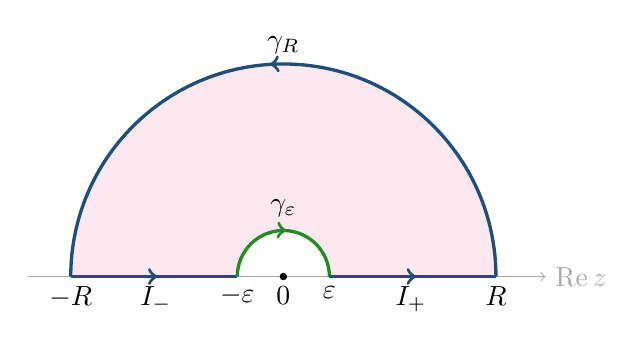
\begin{tikzpicture}[scale=0.9,
 decoration={markings,mark=at position 0.52 with {\arrow{>}}}]
 \fill[lightpink] (-3,0) arc[start angle=180,end angle=0,radius=3]
 --(0.65,0) arc[start angle=0,end angle=180,radius=0.65]--cycle;
 \draw[gray!65,->] (-3.6,0)--(3.7,0) node[right]{$\Real z$};
 \draw[very thick,courseblue,postaction={decorate}] (-3,0)--(-0.65,0);
 \draw[very thick,ForestGreen,postaction={decorate}] (-0.65,0)
 arc[start angle=180,end angle=0,radius=0.65];
 \draw[very thick,courseblue,postaction={decorate}] (0.65,0)--(3,0);
 \draw[very thick,courseblue,postaction={decorate}] (3,0)
 arc[start angle=0,end angle=180,radius=3];
 \node[below] at (-3,0){$-R$};\node[below] at (3,0){$R$};
 \node[below] at (-0.65,0){$-\varepsilon$};
 \node[below] at (0.65,0){$\varepsilon$};
 \fill (0,0) circle(1.5pt) node[below]{$0$};
 \node[above] at (0,3){$\gamma_R$};
 \node[above] at (0,0.7){$\gamma_\varepsilon$};
 \node[below] at (-1.8,0){$I_-$};\node[below] at (1.8,0){$I_+$};
\end{tikzpicture}
\end{center}
For this contour we have
\begin{equation}\label{eq:indented}
 \int_{I_-}f+\int_{\gamma_\varepsilon}f+
 \int_{I_+}f+\int_{\gamma_R}f=0.
\end{equation}
Here is a direct justification using facts already proved, without
assuming a general version of Cauchy's theorem for arbitrary regions.
The exponential series gives
\begin{equation}\label{eq:split}
 f(z)=-\frac{i}{z}+E(z),\qquad
 E(z)=-\sum_{n=2}^{\infty}\frac{i^n z^{n-2}}{n!}
 =\frac12+\frac{iz}{6}-\frac{z^2}{24}+\cdots.
\end{equation}
The series for $E$ converges everywhere. Integrating it term by term
gives an entire primitive of $E$, so $\int_\Gamma E=0$. Also,
\[
 \int_{I_-}\frac{dz}{z}+\int_{I_+}\frac{dz}{z}
 =\log\frac{\varepsilon}{R}+\log\frac{R}{\varepsilon}=0,
\]
while the two semicircles contribute
\[
 \int_{\gamma_\varepsilon}\frac{dz}{z}=\int_\pi^0 i\,d\theta=-i\pi,
 \qquad
 \int_{\gamma_R}\frac{dz}{z}=\int_0^\pi i\,d\theta=i\pi.
\]
Thus $\int_\Gamma dz/z=0$, and \eqref{eq:split} proves
\eqref{eq:indented}.


\subsection{Estimating the arcs and taking limits}
\textbf{The large semicircle.} In the closed upper half-plane,
$|e^{iz}|=e^{-\Imag z}\leq1$, so $|1-e^{iz}|\leq2$.
On $\gamma_R$, therefore, $|f(z)|\leq2/R^2$. The ML estimate gives
\begin{equation}\label{eq:large-arc}
 \left|\int_{\gamma_R}f\right|
 \leq\frac{2}{R^2}\,\pi R=\frac{2\pi}{R}\longrightarrow0
 \qquad(R\to\infty).
\end{equation}

\textbf{The small semicircle.} Use \eqref{eq:split}. Since
$\gamma_\varepsilon$ goes clockwise, its angle decreases from $\pi$ to $0$:
\begin{align*}
 \int_{\gamma_\varepsilon}f(z)\,dz
 &=\int_\pi^0\frac{-i}{\varepsilon e^{i\theta}}
       i\varepsilon e^{i\theta}\,d\theta
       +\int_{\gamma_\varepsilon}E(z)\,dz\\
 &=-\pi+\int_{\gamma_\varepsilon}E(z)\,dz.
\end{align*}
Since $E$ is entire, it is continuous on the compact closed unit disc.
Hence there is a constant $M$ such that
$|E(z)|\leq M$ for $|z|\leq1$. For $0<\varepsilon\leq1$,
\[
 \left|\int_{\gamma_\varepsilon}E(z)\,dz\right|
 \leq M\pi\varepsilon\longrightarrow0.
\]
Consequently,
\begin{equation}\label{eq:small-arc}
 \lim_{\varepsilon\to0^+}\int_{\gamma_\varepsilon}f=-\pi.
\end{equation}

\textbf{The real intervals.} Their sum is
\begin{align*}
 \int_{I_-}f+\int_{I_+}f
 &=\int_{-R}^{-\varepsilon}\frac{1-e^{ix}}{x^2}\,dx
   +\int_\varepsilon^R\frac{1-e^{ix}}{x^2}\,dx\\
 &=2\int_\varepsilon^R\frac{1-\cos x}{x^2}\,dx.
\end{align*}
The real parts add because $(1-\cos x)/x^2$ is even, and the imaginary
parts cancel because $\sin x/x^2$ is odd. Substitution
into \eqref{eq:indented} yields
\[
 2\int_\varepsilon^R\frac{1-\cos x}{x^2}\,dx
 =-\int_{\gamma_\varepsilon}f-\int_{\gamma_R}f.
\]
First let $R\to\infty$ using \eqref{eq:large-arc}, and then let
$\varepsilon\to0^+$ using \eqref{eq:small-arc}. We obtain
\[
 2\int_0^\infty\frac{1-\cos x}{x^2}\,dx=\pi,
\]
which proves \eqref{eq:cosine-goal}.

\section{Integrating holomorphic functions along continuous curves}
% Handwritten Lecture 15, pages 5--7; Lecture 16, pages 1--3.
So far, we have defined contour integrals for piecewise continuously
differentiable paths. We now extend the definition to an arbitrary
\emph{continuous} curve $\gamma\colon[a,b]\to U$, provided that the
integrand $f$ is holomorphic on the open set $U$.

The idea is to use local primitives. If $f$ has a primitive $g$ on all
of $U$, endpoint evaluation suggests the definition
\[
 \int_\gamma f(z)\,dz=g\bigl(\gamma(b)\bigr)-g\bigl(\gamma(a)\bigr).
\]
In general, a global primitive need not exist. We instead divide the
curve into finitely many pieces, each lying in a disc on which $f$ has
a primitive, and add the corresponding endpoint differences.

\subsection{On compact sets}

For our purposes, a subset $K\subseteq\C$ is \textbf{compact} if it is
closed and bounded. Recall that $U\subseteq\C$ is \textbf{open} if, for
every $z\in U$, there is an $r>0$ such that $D(z,r)\subseteq U$.

\begin{lemma}\label{lem:finite-subcover}
Let $K\subseteq\C$ be compact. Any collection
$\{U_\alpha\}_{\alpha\in I}$ of open sets whose union contains $K$
(an \emph{open cover} of $K$) has a finite subcollection whose union
still contains $K$. In other words, there are
$\alpha_1,\ldots,\alpha_n\in I$ such that
\[
 K\subseteq U_{\alpha_1}\cup\cdots\cup U_{\alpha_n}.
\]
The subcollection may be empty when $K=\varnothing$.
\end{lemma}
\begin{proof}
If $K$ is empty, the empty subcollection suffices. Otherwise, suppose
that no finite subcollection covers $K$. Since $K$ is bounded, it is
contained in a closed square $Q_0$. Divide $Q_0$ into four equal closed
squares. For at least one of these squares, say $Q_1$, the set
$K\cap Q_1$ cannot be covered by finitely many of the $U_\alpha$;
otherwise, combining four finite subcollections would cover $K$.

Repeat this construction to obtain nested closed squares
\[
 Q_0\supseteq Q_1\supseteq Q_2\supseteq\cdots,
 \qquad \operatorname{diam}(Q_n)=2^{-n}\operatorname{diam}(Q_0),
\]
such that each $K\cap Q_n$ has no finite subcover. In particular, each
intersection is nonempty, so choose $z_n\in K\cap Q_n$. For $m\geq n$,
both $z_m$ and $z_n$ lie in $Q_n$, and hence
$|z_m-z_n|\leq\operatorname{diam}(Q_n)$. Thus $(z_n)$ is Cauchy and
converges to some $z\in\C$. Since $K$ is closed, $z\in K$.
Also, each $Q_n$ is closed and contains the tail of the sequence, so
$z\in Q_n$ for every $n$.

Choose $\alpha\in I$ with $z\in U_\alpha$. Since $U_\alpha$ is open,
there is an $r>0$ such that $D(z,r)\subseteq U_\alpha$. For sufficiently
large $n$, $\operatorname{diam}(Q_n)<r$. As $z\in Q_n$, this implies
\[
 K\cap Q_n\subseteq Q_n\subseteq D(z,r)\subseteq U_\alpha.
\]
Thus a single member of the cover covers $K\cap Q_n$, a contradiction.
\end{proof}

\begin{exercise}
Suppose $\gamma\colon[a,b]\to\C$ is continuous. Show that it has compact image.
\end{exercise}

\subsection{A uniform neighbourhood of a compact set}
\begin{lemma}\label{lem:compact-neighbourhood}
Let $U\subseteq\C$ be open and $K\subseteq U$ compact. There is an $r>0$
such that $D(z,r)\subseteq U$ for every $z\in K$, where
$D(z,r)=\{w\in\C:|w-z|<r\}$.
\end{lemma}

Informally, a compact subset of an open set stays a \textit{uniform} positive
distance away from the complement of the open set.


\begin{proof}
If $K$ is empty, any $r>0$ works. Otherwise, for each $z\in K$,
openness of $U$ gives a number $r_z>0$ such that
$D(z,2r_z)\subseteq U$. The smaller discs
$\{D(z,r_z):z\in K\}$ form an open cover of $K$. By
Lemma~\ref{lem:finite-subcover}, finitely many suffice:
\[
 K\subseteq\bigcup_{j=1}^n D(z_j,r_{z_j}).
\]
Set $r=\min\{r_{z_1},\ldots,r_{z_n}\}>0$.

Given $z\in K$, choose $j$ with $|z-z_j|<r_{z_j}$. If $w\in D(z,r)$,
the triangle inequality gives
\[
 |w-z_j|\leq |w-z|+|z-z_j|
 <r+r_{z_j}\leq2r_{z_j}.
\]
Hence $w\in D(z_j,2r_{z_j})\subseteq U$. Thus $D(z,r)\subseteq U$
for every $z\in K$, as required.
\end{proof}

\begin{lemma}[A chain of discs along a curve]\label{lem:disc-chain}
Let $\gamma\colon[a,b]\to U$ be continuous, with $U$ open and $a<b$.
There exist a subdivision
\[
 a=a_0<a_1<\cdots<a_n=b
\]
and open discs $D_0,\ldots,D_{n-1}\subseteq U$ such that
$\gamma([a_j,a_{j+1}])\subseteq D_j$ for every $j$.
\end{lemma}
\begin{proof}
The image $K=\gamma([a,b])$ is compact. By
Lemma~\ref{lem:compact-neighbourhood}, choose $r>0$ such that
$D(z,r)\subseteq U$ for every $z\in K$.
Also, $\gamma$ is uniformly continuous on $[a,b]$. Thus there is
$\delta>0$ such that
\[
 s,t\in[a,b],\quad |s-t|<\delta\quad\Longrightarrow\quad
 |\gamma(s)-\gamma(t)|<r/2.
\]
Choose a subdivision with $a_{j+1}-a_j<\delta$, and set
$D_j=D(\gamma(a_j),r)$. For $t\in[a_j,a_{j+1}]$,
$|\gamma(t)-\gamma(a_j)|<r/2$, so the whole subcurve lies in $D_j$.
\end{proof}

\begin{center}
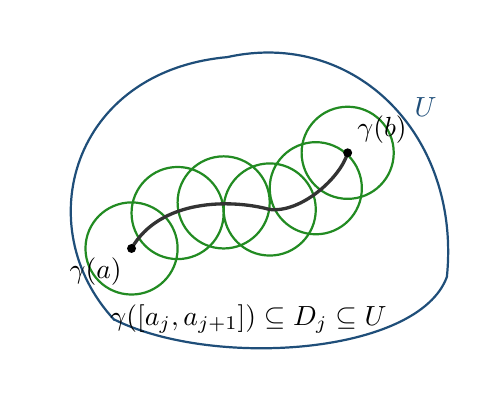
\begin{tikzpicture}[scale=0.9]
 \draw[thick,courseblue] (-0.9,-1.2) .. controls (-2.1,0.1) and (-1.5,2.3)
 .. (0.7,2.5) .. controls (2.5,2.9) and (4,1.4) .. (3.8,-0.6)
 .. controls (3.4,-1.7) and (0.5,-1.9) .. cycle;
 \node[courseblue] at (3.5,1.8){$U$};
 \foreach \x/\y in {-0.65/-0.2,0/0.3,0.65/0.45,1.3/0.35,1.95/0.65,2.4/1.15}
 {\draw[ForestGreen,thick] (\x,\y) circle (0.65);}
 \draw[very thick,darkgray] (-0.65,-0.2) .. controls (-0.25,0.5) and (0.75,0.5)
 .. (1.3,0.35) .. controls (1.75,0.3) and (2.3,0.8) .. (2.4,1.15);
 \fill (-0.65,-0.2) circle (1.8pt) node[below left]{$\gamma(a)$};
 \fill (2.4,1.15) circle (1.8pt) node[above right]{$\gamma(b)$};
 \node at (1,-1.2){$\gamma([a_j,a_{j+1}])\subseteq D_j\subseteq U$};
\end{tikzpicture}
\end{center}

\begin{tcolorbox}[
 enhanced,
 unbreakable,
 colback=lightyellow,
 colframe=warningyellow,
 boxrule=0.7pt,
 arc=2pt,
 left=6pt,
 right=6pt,
 top=5pt,
 bottom=5pt
]
\textbf{Definition (Partition).} Let $\gamma\colon[a,b]\to U$ be
continuous, with $U$ open and $a<b$. Write
\[
 P:=\{a_0,\ldots,a_n\},\qquad a=a_0<\cdots<a_n=b,
\]
for a \emph{subdivision of $[a,b]$}. As in
Lemma~\ref{lem:disc-chain}, we call the data
\[
 \mathscr{D}:=\bigl(P,D_0,\ldots,D_{n-1}\bigr)
\]
a \emph{partition of $\gamma$} if each
$D_j$ is an open disc contained in $U$ with
$\gamma([a_j,a_{j+1}])\subseteq D_j$.
We call $P$ the \emph{underlying subdivision} of $\mathscr{D}$.
\end{tcolorbox}

\subsection{Definition by local primitives}
\begin{definition}\label{def:continuous-integral}
Let $f$ be holomorphic on an open set $U$, and let
$\gamma\colon[a,b]\to U$ be continuous, with $a\leq b$.
If $a<b$, choose a partition $\mathscr{D}$ as above. On each $D_j$,
choose a primitive $g_j$ of $f$, which exists by Cauchy's theorem on
a disc. Define
\begin{equation}\label{eq:continuous-integral}
 \boxed{\displaystyle
 \int_\gamma f(z)\,dz
 =\sum_{j=0}^{n-1}\left[
 g_j\bigl(\gamma(a_{j+1})\bigr)-g_j\bigl(\gamma(a_j)\bigr)
 \right].}
\end{equation}
If $a=b$, define the integral to be zero.
\end{definition}

\begin{remark}
This definition uses the continuity of the curve and the holomorphicity
of $f$. No derivative of $\gamma$ is needed.
\end{remark}

\begin{proposition}\label{prop:well-defined}
The value in \eqref{eq:continuous-integral} is independent of the
partition $\mathscr{D}$ and the chosen local primitives. For a piecewise
continuously differentiable path, it agrees with the usual contour integral.
\end{proposition}
\begin{proof}
If $a=b$, our definition and the usual contour integral both give zero.
We therefore assume $a<b$.

\textbf{Choice of primitive.} If $g$ and $h$ are primitives of $f$ on
one disc $D$, then $(g-h)'=0$. Since $D$ is connected, $g-h$ is constant.
Consequently, for any $w_0,w_1\in D$,
\[
 g(w_1)-g(w_0)=h(w_1)-h(w_0).
\]

\textbf{Possible changes of partition.}
Recall that $\mathscr{D}$ consists of subdivision points \emph{and}
one disc for each subinterval. There are two basic changes to consider:
\begin{enumerate}
 \item \emph{Insert a subdivision point.} Replace $[a_j,a_{j+1}]$ by
 $[a_j,c]$ and $[c,a_{j+1}]$, where $a_j<c<a_{j+1}$. We may use the
 same disc $D_j$ for both pieces, since both subcurves still lie in $D_j$.
 Repeating this operation is called a \emph{refinement of the subdivision}.
 \item \emph{Change a disc.} Keep the subdivision points fixed and
 replace $D_j$ by another open disc $\widetilde D_j\subseteq U$ containing
 the entire subcurve $\gamma([a_j,a_{j+1}])$. The discs need not contain
 one another; it is enough that both contain this subcurve.
\end{enumerate}
One may also remove or move subdivision points, provided the resulting
data still form a partition of $\gamma$. For example, removing a point
requires a disc in $U$ containing the whole merged subcurve. We will
compare such changes by refining both subdivisions to a common one.

\begin{center}
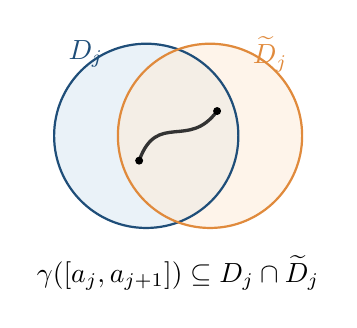
\begin{tikzpicture}[scale=0.9]
 \fill[lightblue] (-0.45,0) circle (1.3);
 \fill[lightorange,fill opacity=0.55] (0.45,0) circle (1.3);
 \draw[thick,courseblue] (-0.45,0) circle (1.3);
 \draw[thick,orangeframe] (0.45,0) circle (1.3);
 \draw[very thick,darkgray] (-0.55,-0.35)
 .. controls (-0.3,0.35) and (0.15,-0.2) .. (0.55,0.35);
 \fill (-0.55,-0.35) circle (1.6pt);
 \fill (0.55,0.35) circle (1.6pt);
 \node[courseblue] at (-1.3,1.15){$D_j$};
 \node[orangeframe] at (1.3,1.15){$\widetilde D_j$};
 \node[below] at (0,-1.55)
 {$\gamma([a_j,a_{j+1}])\subseteq D_j\cap\widetilde D_j$};
\end{tikzpicture}
\end{center}

\textbf{What is a common refinement?}
Given two subdivisions $P=\{a_0,\ldots,a_n\}$ and
$Q=\{b_0,\ldots,b_m\}$ of $[a,b]$, list all their points in increasing
order, counting a point only once if it occurs in both:
\[
 P\cup Q=\{s_0,\ldots,s_N\},\qquad a=s_0<\cdots<s_N=b.
\]
This is their \emph{common refinement}: it is obtained from either
subdivision by inserting points. Each new subinterval
$[s_k,s_{k+1}]$ lies in one subinterval of $P$ and one of $Q$.

\begin{center}
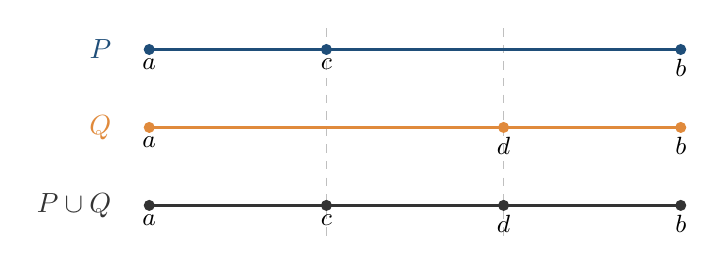
\begin{tikzpicture}[x=0.9cm,y=0.9cm]
 \draw[gray!50,dashed] (2.5,0.3)--(2.5,-2.65);
 \draw[gray!50,dashed] (5,0.3)--(5,-2.65);
 \draw[thick,courseblue] (0,0)--(7.5,0);
 \draw[thick,orangeframe] (0,-1.1)--(7.5,-1.1);
 \draw[thick,darkgray] (0,-2.2)--(7.5,-2.2);
 \node[left,courseblue] at (-0.4,0){$P$};
 \node[left,orangeframe] at (-0.4,-1.1){$Q$};
 \node[left,darkgray] at (-0.4,-2.2){$P\cup Q$};
 \foreach \x/\lab in {0/a,2.5/c,7.5/b}
 {\fill[courseblue] (\x,0) circle (2pt);
  \node[below,font=\small] at (\x,0){$\lab$};}
 \foreach \x/\lab in {0/a,5/d,7.5/b}
 {\fill[orangeframe] (\x,-1.1) circle (2pt);
  \node[below,font=\small] at (\x,-1.1){$\lab$};}
 \foreach \x/\lab in {0/a,2.5/c,5/d,7.5/b}
 {\fill[darkgray] (\x,-2.2) circle (2pt);
  \node[below,font=\small] at (\x,-2.2){$\lab$};}
\end{tikzpicture}
\end{center}

The common refinement aligns the subdivision points; it does not yet
make the disc choices identical. Refine each partition by retaining
its own original disc on every smaller piece. Thus each new subcurve
lies in both an inherited disc $D_j$ from the first partition and an
inherited disc $\widetilde D_\ell$ from the second:
\[
 \gamma([s_k,s_{k+1}])\subseteq D_j\cap\widetilde D_\ell.
\]
We can therefore compare the two primitive increments on this intersection.

\textbf{Refinement of the partition.}
We now check that the changes just described preserve the defining sum.
Insert $c\in(a_j,a_{j+1})$, keeping the disc $D_j$ and its primitive
$g_j$ on both new pieces. Write
\[
 u=\gamma(a_j),\qquad v=\gamma(c),\qquad w=\gamma(a_{j+1}).
\]
The old contribution is $g_j(w)-g_j(u)$, whereas the two new
contributions add to
\begin{align*}
 [g_j(v)-g_j(u)]+[g_j(w)-g_j(v)]
 &=g_j(w)-g_j(u).
\end{align*}
The two values at the inserted point cancel. All other terms in the
sum are unchanged, so inserting one point preserves the sum. By
repeating this argument, any finite refinement preserves it. If we
choose different primitives on the new pieces, the first part of the
proof shows that their endpoint differences are the same.

\begin{center}
\begin{minipage}[t]{0.48\linewidth}
\centering
\vspace{0pt}
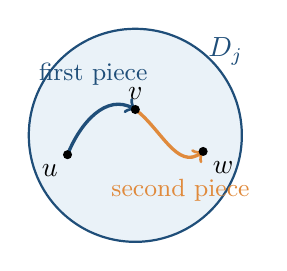
\begin{tikzpicture}[scale=0.82]
 \fill[lightblue] (0,0) circle (1.65);
 \draw[thick,courseblue] (0,0) circle (1.65);
 \node[courseblue] at (1.4,1.3){$D_j$};
 \draw[very thick,courseblue,->] (-1.05,-0.3)
 .. controls (-0.85,0.2) and (-0.45,0.65) .. (0,0.4);
 \draw[very thick,orangeframe,->] (0,0.4)
 .. controls (0.4,0.1) and (0.65,-0.55) .. (1.05,-0.25);
 \fill (-1.05,-0.3) circle (2pt) node[below left]{$u$};
 \fill (0,0.4) circle (2pt) node[above]{$v$};
 \fill (1.05,-0.25) circle (2pt) node[below right]{$w$};
 \node[courseblue,font=\small] at (-0.65,0.95){first piece};
 \node[orangeframe,font=\small] at (0.7,-0.85){second piece};
\end{tikzpicture}
\par\smallskip
{\small One disc and one primitive: the value at $v$ cancels.\par}
\end{minipage}\hfill
\begin{minipage}[t]{0.48\linewidth}
\centering
\vspace{0pt}
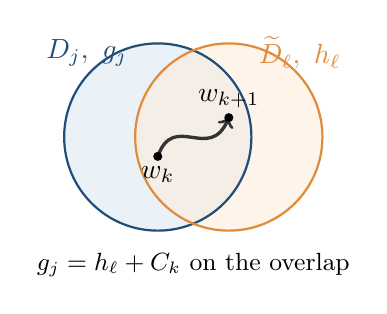
\begin{tikzpicture}[scale=0.82]
 \fill[lightblue] (-0.55,0) circle (1.45);
 \fill[lightorange,fill opacity=0.55] (0.55,0) circle (1.45);
 \draw[thick,courseblue] (-0.55,0) circle (1.45);
 \draw[thick,orangeframe] (0.55,0) circle (1.45);
 \node[courseblue] at (-1.65,1.3){$D_j,\ g_j$};
 \node[orangeframe] at (1.65,1.3){$\widetilde D_\ell,\ h_\ell$};
 \draw[very thick,darkgray,->] (-0.55,-0.3)
 .. controls (-0.3,0.4) and (0.25,-0.4) .. (0.55,0.3);
 \fill (-0.55,-0.3) circle (2pt) node[below]{$w_k$};
 \fill (0.55,0.3) circle (2pt) node[above]{$w_{k+1}$};
 \node[below,font=\small] at (0,-1.65){$g_j=h_\ell+C_k$ on the overlap};
\end{tikzpicture}
\par\smallskip
{\small Two discs: the same constant occurs at both endpoints and cancels.\par}
\end{minipage}
\end{center}

\textbf{Choice of discs and partition.}
Consider any two partitions $\mathscr D$ and $\widetilde{\mathscr D}$,
with subdivisions $P$ and $Q$ and primitives $g_j$ on $D_j$ and
$h_\ell$ on $\widetilde D_\ell$. Refine both to
$P\cup Q=\{s_0,\ldots,s_N\}$, retaining their respective discs and
primitives on each smaller piece. The preceding argument shows that
neither sum changes.

Fix one new subinterval $[s_k,s_{k+1}]$, as in the right-hand diagram
above. It lies in an original
subinterval from each partition, so its image lies in
$D_j\cap\widetilde D_\ell$ for suitable $j$ and $\ell$. This
intersection is nonempty, open, and convex, hence connected. On it,
\[
 (g_j-h_\ell)'=f-f=0,
 \qquad\text{so}\qquad g_j-h_\ell=C_k
\]
for a constant $C_k$. Set $w_k=\gamma(s_k)$ and
$w_{k+1}=\gamma(s_{k+1})$. Both endpoints lie in the intersection,
and therefore
\begin{align*}
 g_j(w_{k+1})-g_j(w_k)
 &=[h_\ell(w_{k+1})+C_k]-[h_\ell(w_k)+C_k]\\
 &=h_\ell(w_{k+1})-h_\ell(w_k).
\end{align*}
Thus the two refined sums agree term by term. Since refinement
preserved each original sum, the original sums agree as well. This
proves independence of the partition, including its disc choices.

\textbf{Agreement with the usual integral.}
Suppose now that $\gamma$ is piecewise continuously differentiable.
Start with any partition used in our definition and insert all the
breakpoints of $\gamma$. The defining sum is unchanged. Denote the
refined subdivision by $a=t_0<\cdots<t_M=b$, and let $G_k$ be the
inherited primitive on a disc containing $\gamma([t_k,t_{k+1}])$.

On each of these pieces, the usual fundamental theorem for a
primitive applies:
\[
 \int_{\gamma|_{[t_k,t_{k+1}]}} f(z)\,dz
 =G_k(\gamma(t_{k+1}))-G_k(\gamma(t_k)).
\]
\begin{center}
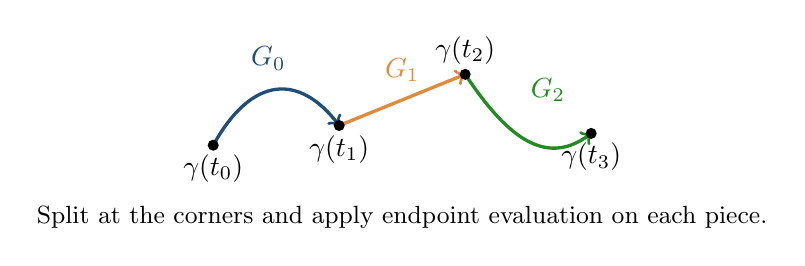
\begin{tikzpicture}[x=1cm,y=1cm]
 \draw[very thick,courseblue,->] (0,0)
 .. controls (0.5,0.9) and (1.1,0.9) .. (1.6,0.25);
 \draw[very thick,orangeframe,->] (1.6,0.25)--(3.2,0.9);
 \draw[very thick,ForestGreen,->] (3.2,0.9)
 .. controls (3.7,0.15) and (4.2,-0.3) .. (4.8,0.15);
 \fill (0,0) circle (2pt) node[below]{$\gamma(t_0)$};
 \fill (1.6,0.25) circle (2pt) node[below]{$\gamma(t_1)$};
 \fill (3.2,0.9) circle (2pt) node[above]{$\gamma(t_2)$};
 \fill (4.8,0.15) circle (2pt) node[below]{$\gamma(t_3)$};
 \node[courseblue] at (0.7,1.1){$G_0$};
 \node[orangeframe] at (2.4,0.95){$G_1$};
 \node[ForestGreen] at (4.25,0.7){$G_2$};
 \node[below,font=\small] at (2.4,-0.65)
 {Split at the corners and apply endpoint evaluation on each piece.};
\end{tikzpicture}
\end{center}
Adding these identities, additivity of the usual contour integral
shows that it equals our defining sum.
\end{proof}

\begin{corollary}[Endpoint evaluation]
If $f$ has a primitive $g$ on $U$, then for every continuous curve
$\gamma\colon[a,b]\to U$,
\[
 \int_\gamma f(z)\,dz=g(\gamma(b))-g(\gamma(a)).
\]
In particular, the integral is zero on every closed continuous curve in
$U$. Thus Cauchy's theorem on a disc also holds for continuous curves.
\end{corollary}
\begin{proof}
Use the restrictions of $g$ as the local primitives. The sum telescopes.
\end{proof}
The integral is linear in $f$, additive when curves are concatenated,
and changes sign when the orientation is reversed. Each property follows
directly from the endpoint differences in \eqref{eq:continuous-integral}.

\end{document}
